\appendixsection{Состав backend-сервисов}

В приложении приведена таблица с кратким описанием сервисов. Она позволяет наглядно показать состав backend-платформы и зону ответственности каждого сервиса.

\begingroup
\TableFontPt{12}
\begin{longtable}{|
  >{\raggedright\arraybackslash}p{0.15\columnwidth}|
  >{\raggedright\arraybackslash}p{0.21\columnwidth}|
  >{\raggedright\arraybackslash}p{0.16\columnwidth}|
  >{\raggedright\arraybackslash}p{0.34\columnwidth}|}
\caption{Состав backend-сервисов CoachLink}\label{tab:appendix-service-map}\\
\hline
\begin{minipage}[b]{\linewidth}\raggedright
Сервис
\end{minipage} & \begin{minipage}[b]{\linewidth}\raggedright
Назначение
\end{minipage} & \begin{minipage}[b]{\linewidth}\raggedright
Хранилище
\end{minipage} & \begin{minipage}[b]{\linewidth}\raggedright
Основные взаимодействия
\end{minipage} \\
\hline
\endhead
\hline
\endlastfoot
API Gateway & Единая точка входа, JWT-проверка, reverse proxy & Без собственной БД & Принимает внешние REST-запросы и маршрутизирует их на внутренние сервисы \\ \hline
Auth Service & Регистрация, login, refresh/logout, выдача JWT & PostgreSQL & Публикует \path|coachlink.user.registered| в NATS \\ \hline
User Service & Профили, заявки, связи, группы, поиск & PostgreSQL & Принимает событие регистрации, предоставляет внутренние проверки доступа \\ \hline
Training Service & Планы, шаблоны, назначения, отчёты, статусы & PostgreSQL & Публикует события назначений и отчётов, предоставляет данные аналитике \\ \hline
Notification Service & Уведомления, unread count, FCM-токены & PostgreSQL & Подписывается на события NATS \\ \hline
Analytics Service & Summary, progress, coach overview & Stateless & Получает данные из Training Service и User Service \\ \hline
AI Service & Рекомендации по последним отчётам спортсмена & Stateless & Проверяет связь через User Service, получает данные из Analytics Service, обращается к Ollama \\ \hline
\end{longtable}
\endgroup

AI Service и Analytics Service реализованы как stateless-сервисы. Они не владеют собственными предметными данными и формируют результат на основе данных других сервисов.

\appendixsection{Группы публичного API}

В приложении представлена таблица публичных API-групп. Полный перечень endpoints содержится в \passthrough{\lstinline!docs/api/openapi.yaml!}, а в тексте диплома используется сгруппированное представление.

\begingroup
\TableFontPt{12}
\begin{longtable}{|
  >{\raggedright\arraybackslash}p{0.18\columnwidth}|
  >{\raggedright\arraybackslash}p{0.44\columnwidth}|
  >{\raggedright\arraybackslash}p{0.28\columnwidth}|}
\caption{Группы публичного API и их назначение}\label{tab:appendix-api-groups}\\
\hline
\begin{minipage}[b]{\linewidth}\raggedright
Группа API
\end{minipage} & \begin{minipage}[b]{\linewidth}\raggedright
Примеры endpoints
\end{minipage} & \begin{minipage}[b]{\linewidth}\raggedright
Назначение
\end{minipage} \\
\hline
\endhead
\hline
\endlastfoot
Auth API & POST \path|/api/v1/auth/register|,\linebreak POST \path|/api/v1/auth/login| & Регистрация и аутентификация пользователей \\ \hline
User API & \path|/api/v1/users/me|,\linebreak \path|/api/v1/users/search| & Профили, поиск, заявки, связи, группы \\ \hline
Training API & \path|/api/v1/training/plans|,\linebreak \path|/api/v1/training/assignments/{id}/report| & Планы, назначения, отчёты и шаблоны \\ \hline
Notification API & \path|/api/v1/notifications|,\linebreak \path|/api/v1/notifications/{id}/read| & Уведомления и отметка прочтения \\ \hline
Analytics API & \path|/api/v1/analytics/athletes/{id}/summary|,\linebreak \path|/api/v1/analytics/coach/overview| & Агрегация тренировочных данных \\ \hline
AI API & POST \path|/api/v1/ai/athletes/{id}/recommendations| & Рекомендации по последним отчётам спортсмена \\ \hline
System API & \path|/health|,\linebreak \path|/api/v1/health| & Проверка доступности сервисов \\ \hline
\end{longtable}
\endgroup


\appendixsection{Примеры JSON-запросов и ответов}

Примеры API отражают backend-логику и не зависят от особенностей мобильного интерфейса. В качестве репрезентативных примеров приведены отправка отчёта и получение AI-рекомендации.

\subsection*{Пример отправки отчёта о тренировке}

\begin{lstlisting}
{
  "content": "Выполнил кросс спокойно, последние 2 км немного быстрее.",
  "duration_minutes": 46,
  "perceived_effort": 6,
  "max_heart_rate": 174,
  "avg_heart_rate": 151,
  "distance_km": 8.0
}
\end{lstlisting}

Пример показывает тело запроса для endpoint \passthrough{\lstinline!POST /api/v1/training/assignments/\{assignmentId\}/report!}. Идентификатор назначения передаётся в path-параметре, а отчёт хранится в структурированном виде. В отличие от сообщения в мессенджере, backend может использовать поля отчёта для аналитики: рассчитывать недельный объём, длительность, дистанцию, среднюю воспринимаемую нагрузку и пульсовые показатели.

\subsection*{Пример ответа на создание отчёта}

\begin{lstlisting}
{
  "id": "7f9ef6c3-0fd9-4cfd-a69d-d3d1b65a157d",
  "assignment_id": "2b54c487-0ef3-4e60-8e9a-7f2fdb66c101",
  "athlete_id": "a52d4f18-e218-4d2a-bd4f-01bcb89d01f2",
  "athlete_full_name": "Петров Иван Сергеевич",
  "athlete_login": "ivan-petrov",
  "content": "Выполнил кросс спокойно, последние 2 км немного быстрее.",
  "duration_minutes": 46,
  "perceived_effort": 6,
  "max_heart_rate": 174,
  "avg_heart_rate": 151,
  "distance_km": 8.0,
  "created_at": "2026-04-18T18:30:00Z"
}
\end{lstlisting}

После создания отчёта Training Service публикует событие, на которое подписан Notification Service. Благодаря этому тренер получает уведомление без прямой зависимости между Training Service и способом доставки уведомлений.

\subsection*{Пример запроса AI-рекомендации}

\begin{lstlisting}
{
  "context": "Подготовка к старту на 800 м через два месяца."
}
\end{lstlisting}

\subsection*{Пример ответа AI Service}

Ответ возвращается в формате JSON. Поле \passthrough{\lstinline!content!} содержит фактический текст, сгенерированный моделью \passthrough{\lstinline!gemma3:4b!} по реальной истории тренировок тестового спортсмена.

\begin{lstlisting}
{
  "athlete_id": "a52d4f18-e218-4d2a-bd4f-01bcb89d01f2",
  "type": "recommendations",
  "content": "
  Тенденции
  Средняя продолжительность тренировок — 47 мин, дистанция в последней сессии выросла до 6.4 км против стабильных 5.0 км в предыдущих двух. Воспринимаемая нагрузка — 8/10 в каждой из трёх последних тренировок, максимальный пульс 182 уд/мин зафиксирован в интервальной сессии.

  Риски
  Сочетание высокой субъективной нагрузки (8/10) с ростом объёма и комментарием спортсмена «тяжёлые ноги на последних отрезках» указывает на накопленную усталость. Пульс 182 уд/мин при 100% выполнения заданий — вероятный признак недовосстановления.

  Рекомендации
  1. Следующую интервальную сессию сократить до 6×400 м и провести не ранее чем через 72 часа.
  2. Добавить один восстановительный день с лёгким бегом до 30 мин при пульсе ниже 140.
  3. Удерживать пульс на отрезках ниже 178 уд/мин для контроля интенсивности.
  Модель: gemma3:4b · локально через Ollama · данные: 3 последних отчёта тестового спортсмена
  ",
  "generated_at": "2026-04-18T18:35:00Z",
  "model": "gemma3:4b"
}
\end{lstlisting}

AI-рекомендация является вспомогательной информацией. Она не заменяет решение тренера и не используется как автоматическое назначение тренировочного плана.

\appendixsection{ER-диаграмма основных таблиц}

В приложении приведена расширенная ER-диаграмма, отражающая структуру и связи основных таблиц backend-платформы. В отличие от диаграммы в основном тексте, данное представление включает детализацию полей и типов данных. В микросервисной архитектуре CoachLink таблицы физически распределены по базам данных отдельных сервисов. На рисунке~\ref{fig:er-main-tables} представлена расширенная ER-диаграмма.

\begin{figure}[H]
  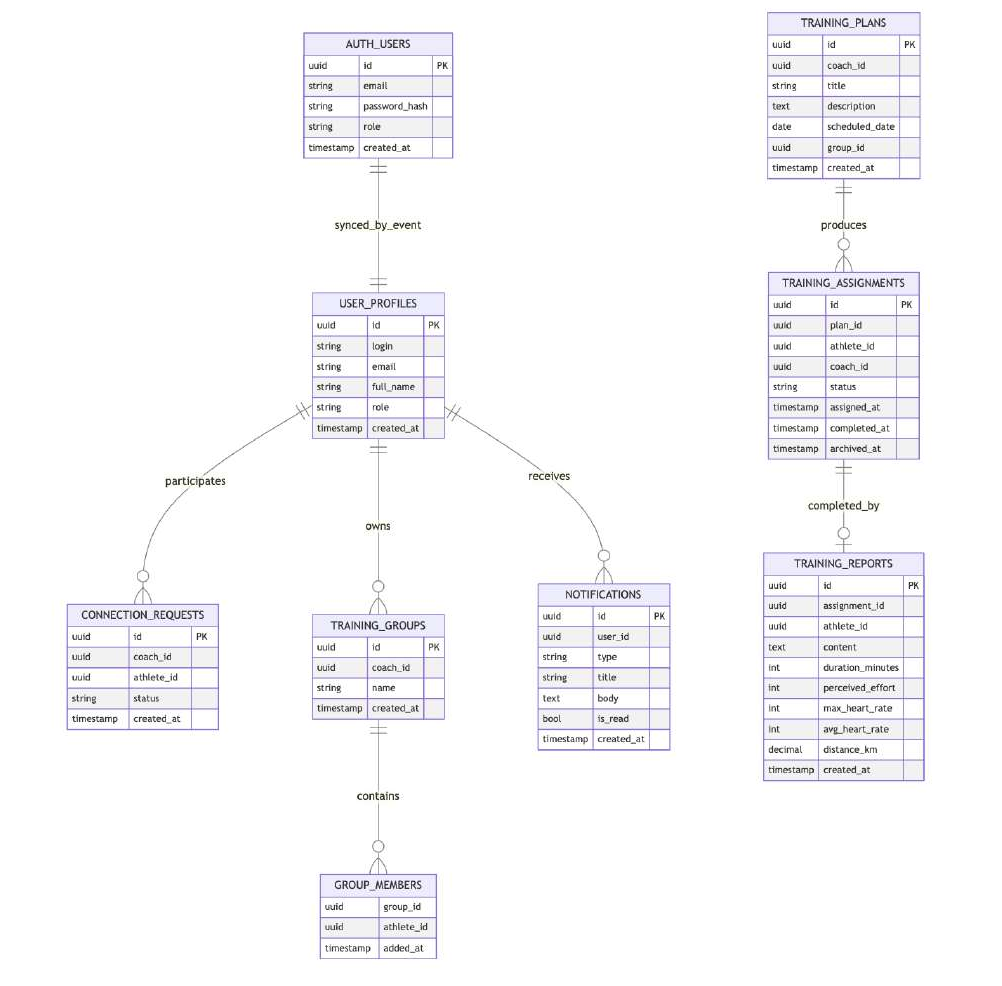
\includegraphics[width=\textwidth]{inc/er-main-tables_cropped.pdf}
  \caption{Расширенная ER-диаграмма основных таблиц платформы CoachLink}
  \label{fig:er-main-tables}
\end{figure}


\appendixsection{События NATS JetStream в backend-платформе}

В приложении приведена таблица событий, используемых для слабосвязанного взаимодействия сервисов.

\begingroup
\TableFontPt{12}
\begin{longtable}{|
  >{\raggedright\arraybackslash}p{0.42\columnwidth}|
  >{\raggedright\arraybackslash}p{0.13\columnwidth}|
  >{\raggedright\arraybackslash}p{0.16\columnwidth}|
  >{\raggedright\arraybackslash}p{0.17\columnwidth}|}
\caption{События NATS JetStream для межсервисного взаимодействия}\label{tab:appendix-nats-events}\\
\hline
\begin{minipage}[b]{\linewidth}\raggedright
Событие
\end{minipage} & \begin{minipage}[b]{\linewidth}\raggedright
Источник
\end{minipage} & \begin{minipage}[b]{\linewidth}\raggedright
Получатель
\end{minipage} & \begin{minipage}[b]{\linewidth}\raggedright
Назначение
\end{minipage} \\
\hline
\endhead
\hline
\endlastfoot
\path|coachlink.user.registered| & Auth Service & User Service & Создание профиля пользователя \\ \hline
\path|coachlink.connection.requested| & User Service & Notification Service & Уведомление тренера о новой заявке \\ \hline
\path|coachlink.connection.accepted| & User Service & Notification Service & Уведомление спортсмена о принятии заявки \\ \hline
\path|coachlink.connection.rejected| & User Service & Notification Service & Уведомление спортсмена об отклонении заявки \\ \hline
\path|coachlink.group.athlete_added| & User Service & Notification Service & Уведомление о добавлении в группу \\ \hline
\path|coachlink.group.athlete_removed| & User Service & Notification Service & Уведомление об удалении из группы \\ \hline
\path|coachlink.training.assigned| & Training Service & Notification Service & Уведомление о назначенной тренировке \\ \hline
\path|coachlink.training.deleted| & Training Service & Notification Service & Уведомление об удалении назначения \\ \hline
\path|coachlink.report.submitted| & Training Service & Notification Service & Уведомление тренера о новом отчёте \\ \hline
\end{longtable}
\endgroup

Названия событий взяты из общего пакета \passthrough{\lstinline!pkg/events!} и соответствуют текущей событийной модели платформы.

\appendixsection{Таблица тестирования}

Таблица тестирования отражает фактически подтверждённые результаты запусков.

\begingroup
\TableFontPt{12}
\begin{longtable}{|
  >{\raggedright\arraybackslash}p{0.23\columnwidth}|
  >{\raggedright\arraybackslash}p{0.24\columnwidth}|
  >{\raggedright\arraybackslash}p{0.22\columnwidth}|
  >{\raggedright\arraybackslash}p{0.19\columnwidth}|}
\caption{Уровни тестирования и критерии фиксации результатов}\label{tab:appendix-test-plan}\\
\hline
\begin{minipage}[b]{\linewidth}\raggedright
Уровень тестирования
\end{minipage} & \begin{minipage}[b]{\linewidth}\raggedright
Команда
\end{minipage} & \begin{minipage}[b]{\linewidth}\raggedright
Назначение
\end{minipage} & \begin{minipage}[b]{\linewidth}\raggedright
Статус
\end{minipage} \\
\hline
\endhead
\hline
\endlastfoot
Unit-тесты & make test-unit & Проверка сервисного слоя отдельных микросервисов & 112 тестов пройдено \\ \hline
E2E smoke & make test-e2e & Проверка базового e2e-сценария при поднятой платформе & 19 шагов пройдено \\ \hline
Integration & make\linebreak test-integration & Проверка API Gateway и межсервисных сценариев & 113 проверок пройдено \\ \hline
\end{longtable}
\endgroup